% GNNV — SAIV 2026 oral presentation (10–12 minutes)
% Engine: pdfLaTeX     Build:  latexmk -pdf main.tex
%
% Structure: motivation (graphs across domains) -> contributions ->
%            approach (lifting NNV to GNNs: GCN + GINE) -> results -> tool.
%
% Timing plan (~11:00):
%   1  Title                          0:20
%   2  Graphs across domains          0:50
%   3  What a GNN computes            0:50
%   4  Message passing, step by step  1:10
%   5  The gap (no guarantees)        0:50
%   6  Contributions                  1:00
%   -- Approach --
%   7  NNV + Star sets                0:55
%   8  GraphStar sets                 1:00
%   9  GCN + GINE reachability        0:55
%  10  Pipeline (full figure)         0:35
%  11  Pipeline (stepped)             0:50
%  12  Sound + tractable              0:45
%   -- Results --
%  13  Experimental setup             0:35
%  14  RQ1 robustness at scale        0:45
%  15  RQ2 edge perturbations         0:40
%  16  RQ3 tighter than CORA          0:50
%   -- Closing --
%  17  Tool availability              0:40
%  18  Conclusions                    0:40
%  19  Thank you                      0:15
\documentclass[11pt,aspectratio=169,t]{beamer}

\usetheme{Vanderbilt}
\institutelogo{Vanderbilt_University_logo_transparent.png}

\usepackage{amsmath,amssymb,mathtools}
\usepackage{booktabs}
\usepackage{tikz}
\usetikzlibrary{arrows.meta,positioning,calc,shapes.geometric,backgrounds,fit}

% Semantic brackets + shorthand
\newcommand{\lb}{[\![}
\newcommand{\rb}{]\!]}
\newcommand{\GS}{\Theta_{\mathcal{G}}}
\newcommand{\R}{\mathbb{R}}

% Semantic result colors (match the paper's data figures)
\definecolor{safegreen}{HTML}{2E9E5B}
\definecolor{unsafered}{HTML}{CC4A3F}
\definecolor{steelblue}{HTML}{2E5C8A}
\definecolor{amber}{HTML}{E4A63A}
\newcommand{\good}[1]{\textbf{\textcolor{safegreen}{#1}}}
\newcommand{\bad}[1]{\textbf{\textcolor{unsafered}{#1}}}
\newcommand{\key}[1]{\textbf{\textcolor{VUgoldDark}{#1}}}

% Message-passing stage colours, shared by the message-passing slide and the
% GCN/GINE slide so the two line up visually.
\definecolor{aggcol}{HTML}{2E5C8A}   % aggregate  (steel blue)
\definecolor{combcol}{HTML}{6A4C93}  % combine / update (violet)
\newcommand{\aggr}[1]{\textcolor{aggcol}{#1}}
\newcommand{\comb}[1]{\textcolor{combcol}{#1}}

% callout strip that sits just above the footer
\setbeamercolor{calloutbox}{fg=VUblack, bg=VUgold!25}
\newcommand{\takeaway}[1]{\vfill
  \nointerlineskip%
  \begin{beamercolorbox}[wd=\textwidth, sep=0.6ex, rounded=true]{calloutbox}%
    \small\textcolor{VUgoldDark}{$\blacktriangleright$}~\textbf{#1}%
  \end{beamercolorbox}}

% slide-bottom reference line
\newcommand{\refline}[1]{\par\vfill\nointerlineskip
  {\centering\tiny\color{VUgrey!75} #1\par}\vspace{0.2ex}}

% domain panel for the motivation slide
\newcommand{\dompanel}[4]{%
  % #1 image  #2 title  #3 nodes/edges  #4 task + citation
  \begin{minipage}[t]{0.235\textwidth}\centering
    \colorbox{VUlight}{\parbox{\dimexpr\linewidth-2\fboxsep}{\centering
      \vspace{0.4ex}\includegraphics[height=2.08cm]{#1}\vspace{0.4ex}}}\\[0.7ex]
    {\small\bfseries #2}\\[0.4ex]
    {\scriptsize #3}\\[0.5ex]
    {\scriptsize\itshape\color{VUgoldDark} #4}
  \end{minipage}}

\tikzset{
  gnode/.style={circle, draw=VUblack, thick, fill=VUgold!45, minimum size=7mm, font=\small\bfseries},
  gedge/.style={draw=VUgrey, very thick},
  flow/.style={-{Stealth[length=2.6mm]}, thick, draw=VUgrey},
  % message-passing slide
  vec/.style={draw=VUgrey!70, fill=#1, minimum width=3.6mm, minimum height=2.4mm,
              inner sep=0pt, anchor=south},
  slbl/.style={font=\scriptsize, text=VUgrey},
  stepbox/.style={rectangle, rounded corners=2pt, draw=VUgoldDark, fill=VUgold!16,
                  inner sep=3pt, font=\small},
}

\title{Reachability-Based Formal Verification of Graph Neural Networks with Node and Edge Features}
\date{Symposium on AI Verification (SAIV) 2026}
\author{\textbf{Anne M.~Tumlin}, Ben Wooding, Zhenxuan Shao,\\ Diego Manzanas Lopez, Tyler Derr, Taylor T.~Johnson}
\institute{Vanderbilt University, Nashville, TN, USA}

\makeatletter
\def\insertshortauthor{A. M. Tumlin et al.}
\def\insertshorttitle{Formal Verification of GNNs (GNNV)}
\makeatother

\begin{document}

{\setbeamertemplate{footline}{}\maketitle}

% ===========================================================================
% MOTIVATION
% ===========================================================================

\begin{frame}{GNN Surrogates Across Application Domains}
  \centering
  \dompanel{figures/dom_molecule_flat.png}{Molecules}
    {nodes: atoms\\ edges: bonds (type, order)}{property prediction [1]}\hfill
  \dompanel{figures/dom_protein_flat.png}{Proteins}
    {nodes: residues\\ edges: spatial contacts}{function classification [2]}\hfill
  \dompanel{figures/dom_traffic_crop.png}{Traffic}
    {nodes: intersections\\ edges: roads (speed, load)}{flow forecasting [3]}\hfill
  \dompanel{figures/dom_power_crop.png}{Power Grids}
    {nodes: buses $(P,Q,|V|,\theta)$\\ edges: lines $(g,b)$}{PF, OPF, CFA [4]}
  \vskip1.2ex

  \visible<2->{{\small Different domains, one shared computation:
  \textbf{message passing over node and edge features}.\\[0.4ex]
  \textcolor{VUgoldDark}{\textbf{These predictions drive high-stakes decisions,
  so we need guarantees, not just accuracy.}}}}

  \refline{[1]~Gilmer et al., ICML 2017.\ \ [2]~Morris et al., TUDataset (ICML-W 2020).\ \
           [3]~Jiang \& Luo, ESWA 2022.\ \ [4]~Varbella et al., NeurIPS 2024.\ \
           Images (Wikimedia Commons).}
\end{frame}

\begin{frame}{Graph-Structured Inputs: Node and Edge Feature Matrices}
  \begin{columns}[T,onlytextwidth]
    \begin{column}{0.46\textwidth}
      A graph $\mathcal{G}=(\mathcal{V},\mathcal{E})$ carries
      \begin{itemize}\setlength{\itemsep}{0.2ex}
        \item node features $X \in \R^{N\times d_f}$
        \item edge features $E \in \R^{M\times d_e}$
        \item adjacency $A \in \mathbb{B}^{N\times N}$
      \end{itemize}
      \vskip0.2ex

      \visible<2->{The \key{graph topology} governs which node representations
      interact during message passing; since inputs live on nodes \textbf{and}
      edges, a guarantee must cover both.}
      \vskip0.4ex

      \visible<3->{%
      \begin{block}{Two Task Types}
        \small
        \textbf{node-level:} regress $\hat y_v$\\
        \textbf{graph-level:} classify $\mathcal{G}$
      \end{block}}
    \end{column}
    \begin{column}{0.52\textwidth}
      \centering
      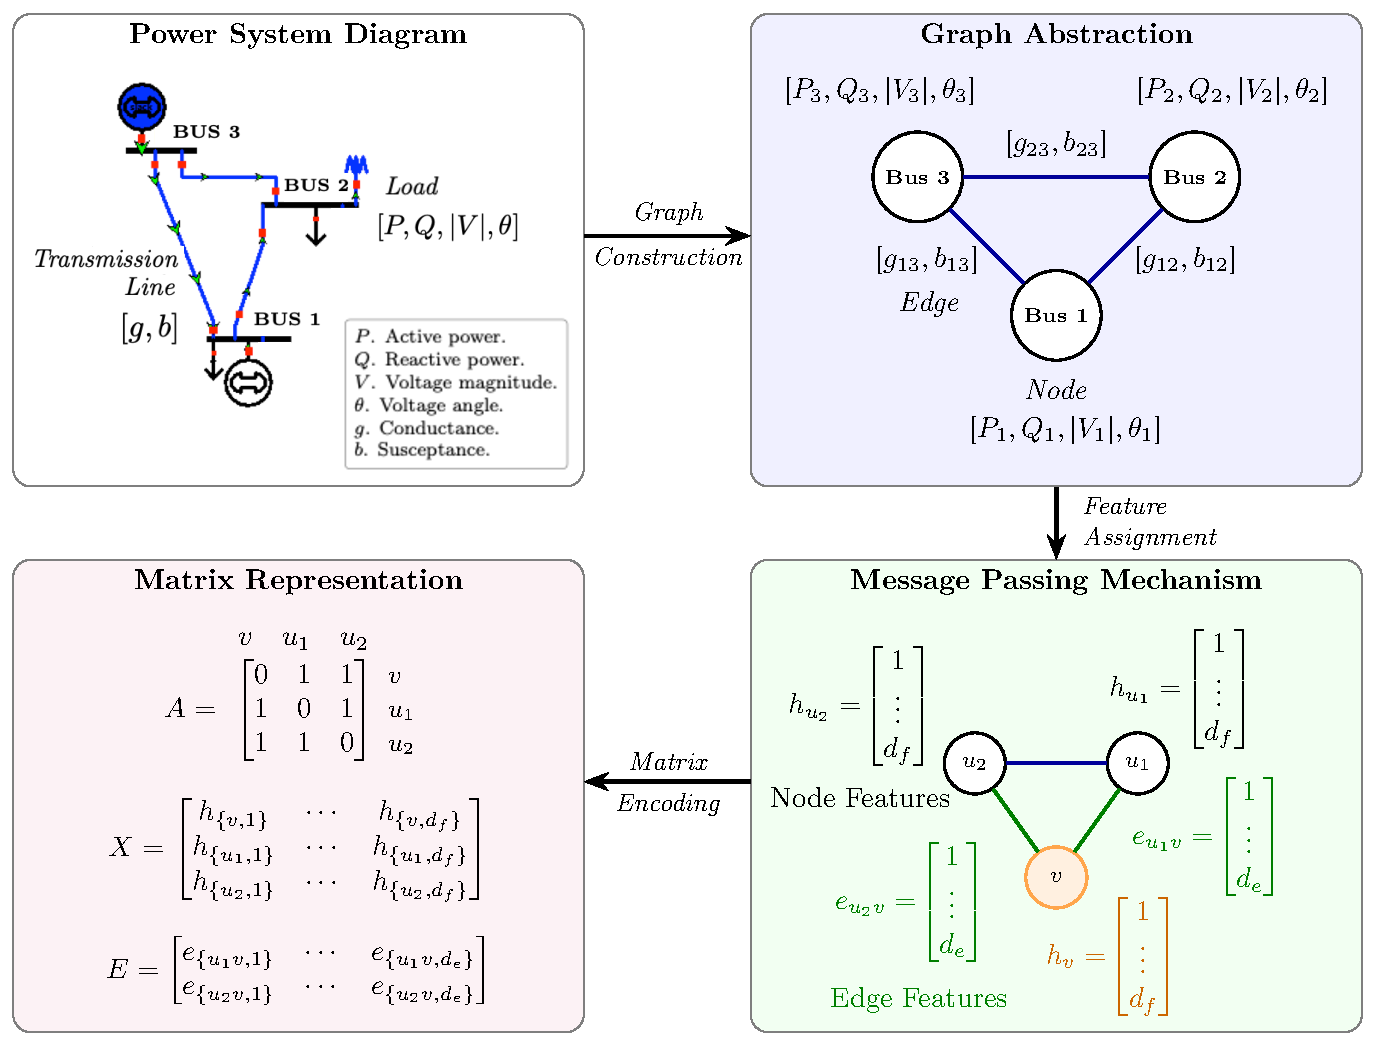
\includegraphics[width=0.92\linewidth]{figures/gnn_construction_v5.pdf}\\[0.3ex]
      {\scriptsize A power grid mapped to a graph. Any domain maps the same
      way.\ \ {\color{VUgrey!75}[our paper, Fig.~1]}}
    \end{column}
  \end{columns}
\end{frame}

\begin{frame}{Message Passing: Message $\to$ Aggregate $\to$ Update}
  \centering
  \begin{tikzpicture}[scale=0.9, transform shape]
    % ================= (a) an irregular graph =================
    \node[font=\small, text=VUgrey, anchor=south] at (1.4,2.25) {\textbf{target node $v$ in its neighbourhood}};
    % neighbours of v, scattered at uneven angles/distances
    \node[gnode, fill=aggcol!30, minimum size=6mm] (u1) at (0.15,1.35) {$u_1$};
    \node[gnode, fill=aggcol!30, minimum size=6mm] (u2) at (-0.35,-0.25) {$u_2$};
    \node[gnode, fill=aggcol!30, minimum size=6mm] (u3) at (1.35,-1.5) {$u_3$};
    \node[gnode, minimum size=7mm] (v) at (1.95,0.35) {$v$};
    % 2-hop node and an unused node (never reaches v within K=1)
    \node[gnode, fill=VUgrey!12, minimum size=5.5mm] (w) at (-1.5,1.9) {$w$};
    \node[gnode, fill=VUgrey!12, minimum size=5.5mm] (q) at (-1.7,0.45) {$q$};
    \node[gnode, fill=VUgrey!12, minimum size=5.5mm] (r) at (0.55,-2.5) {$r$};
    % edges: neighbours interconnect, so it reads as a graph not a layer
    \draw[gedge] (u1)--(v); \draw[gedge] (u2)--(v); \draw[gedge] (u3)--(v);
    \draw[gedge] (u1)--(u2);
    \draw[gedge] (w)--(u1); \draw[gedge] (w)--(q); \draw[gedge] (q)--(u2);
    \draw[gedge] (r)--(u3);
    \node[font=\scriptsize, text=VUgrey!80, anchor=north, align=center] at (-1.3,-1.0)
      {$q$, $r$, $w$: outside\\ $v$'s 1-hop neighbourhood};

    % ================= (b) gather =================
    \visible<2->{
      \draw[-{Stealth[length=2.4mm]}, very thick, VUgoldDark] (u1)--(v);
      \draw[-{Stealth[length=2.4mm]}, very thick, VUgoldDark] (u2)--(v);
      \draw[-{Stealth[length=2.4mm]}, very thick, VUgoldDark] (u3)--(v);
      \node[font=\scriptsize, text=VUgoldDark, anchor=south west] at (1.0,0.9) {$e_{u_1 v}$};
      \node[stepbox, anchor=west] at (3.4,1.6)
        {$m_{uv} = \phi\big(h_u^{(\ell)},\, \textcolor{VUgoldDark}{e_{uv}}\big)$};
      \node[slbl, anchor=north west, text width=4.4cm] at (3.4,1.15)
        {\textcolor{VUgoldDark}{\textbf{1. Message:}} each neighbour's features
         $+$ its \textcolor{VUgoldDark}{edge feature} $e_{uv}$};
    }
    % ================= (c) aggregate =================
    \visible<3->{
      \node[stepbox, anchor=west, draw=aggcol, fill=aggcol!12] at (3.4,-0.2)
        {$\aggr{z_v = \textstyle\sum_{u\in\mathcal{N}(v)} m_{uv}}$};
      \node[slbl, anchor=north west, text width=4.4cm] at (3.4,-0.65)
        {\textbf{\aggr{2. Aggregate:}} an order-invariant sum over neighbours};
    }
    % ================= (d) update / combine =================
    \visible<4->{
      \node[stepbox, anchor=west, draw=combcol, fill=combcol!12] at (3.4,-1.85)
        {$\comb{h_v^{(\ell+1)} = \sigma\big(W z_v + b\big)}$};
      \node[slbl, anchor=north west, text width=4.4cm] at (3.4,-2.3)
        {\textbf{\comb{3. Update}} (combine): a learned map, then ReLU};
    }

    % ================= (e) vectors on the right =================
    \visible<2->{
      \node[font=\small, text=VUgrey, anchor=south] at (10.35,2.3) {\textbf{what node $v$ holds}};
      \foreach \x/\lab in {8.85/$m_{u_1v}$, 9.55/$m_{u_2v}$, 10.25/$m_{u_3v}$}{
        \foreach \i in {0,...,3} {\node[vec=VUgold!45] at (\x, 0.6+\i*0.24) {};}
        \node[font=\scriptsize, text=VUgrey, anchor=north] at (\x+0.09,0.5) {\lab};}
    }
    \visible<3->{
      \node[font=\large, text=aggcol] at (10.9,1.0) {$\Rightarrow$};
      \foreach \i in {0,...,3} {\node[vec=aggcol!45] at (11.45, 0.6+\i*0.24) {};}
      \node[font=\scriptsize, text=VUgrey, anchor=north] at (11.54,0.5) {$z_v$};
    }
    \visible<4->{
      \node[font=\large, text=combcol] at (10.9,-1.15) {$\Downarrow$};
      \foreach \i in {0,...,3} {\node[vec=combcol!40] at (11.45, -1.55+\i*0.24) {};}
      \node[font=\scriptsize, text=VUgrey, anchor=north] at (11.59,-1.62) {$h_v^{(\ell+1)}$};
      \node[font=\small, text=VUgrey, anchor=east, text width=2.9cm, align=right] at (10.65,-1.15)
        {every node updates \textbf{in parallel}};
    }
    % ================= (f) next layer =================
    \visible<5->{
      \draw[-{Stealth[length=2.4mm]}, very thick, unsafered, dashed] (w)--(u1);
      \draw[-{Stealth[length=2.4mm]}, very thick, unsafered, dashed] (q)--(u2);
      \draw[-{Stealth[length=2.4mm]}, very thick, unsafered, dashed] (r)--(u3);
      \node[font=\scriptsize, text=unsafered, anchor=east] at (-1.9,1.35) {layer 2};
    }
  \end{tikzpicture}
  \vfill
  \visible<5->{%
  {\footnotesize After $K$ layers $h_v$ summarises $v$'s \key{$K$-hop
  neighbourhood}, which is also how far a \bad{perturbation} can travel.\par}}
  \vskip0.5ex
  {\centering\tiny\color{VUgrey!75} Gilmer et al., ICML 2017;\ \ Xu et al., ICLR 2019.\par}
\end{frame}

{\setbeamerfont{frametitle}{size=\footnotesize,series=\bfseries}
\begin{frame}{Graph Convolutional Network (GCN) and Graph Isomorphism Network with Edge Features (GINE)}
  \centering
  {\small Same three stages as the previous slide:\ \
   \textbf{message} $\to$
   \aggr{\textbf{aggregate}} $\to$ \comb{\textbf{combine}} (update).\par}
  \vskip-0.3ex

  \begin{columns}[T,onlytextwidth]
    \begin{column}{0.495\textwidth}
      \begin{block}{GCN}
        \small
        \vspace{-3ex}
        \[
          H^{(\ell+1)} = \sigma\big(
          \underbrace{\aggr{\tilde D^{-\frac12}\tilde A \tilde D^{-\frac12}
          H^{(\ell)}}}_{\aggr{\text{aggregate}}}\,
          \underbrace{\comb{W^{(\ell)}}}_{\comb{\text{combine}}}\big)
        \]
        \vspace{-3ex}
        \begin{itemize}
          \setlength{\itemsep}{0.4ex}\footnotesize
          \item \aggr{aggregate}: normalised neighbour average; self-loops
                $\tilde A{=}A{+}I$ fold in $v$'s own state
          \item \comb{combine}: one linear map $W^{(\ell)}$, no MLP;
                \textbf{node features only} ($E$ never enters)
        \end{itemize}
      \end{block}
    \end{column}
    \begin{column}{0.495\textwidth}
      \begin{block}{GINE}
        \small
        \vspace{-3ex}
        \begin{align*}
          \aggr{Z^{(\ell)}} &= \aggr{R^\top\big(S H^{(\ell)} +
             \textcolor{VUgoldDark}{E\,W_e^{(\ell)}} + b_e^{(\ell)}\big)}
             &&\aggr{\text{aggregate}}\\[-0.3ex]
          H^{(\ell+1)} &= \comb{\sigma\big(\sigma(Z^{(\ell)} W_1 + b_1) W_2 + b_2\big)}
             &&\comb{\text{combine}}
        \end{align*}
        \vspace{-4ex}
        \begin{itemize}
          \setlength{\itemsep}{0.3ex}\footnotesize
          \item \aggr{aggregate} gathers ($S$) and scatters ($R^\top$);
                \comb{combine} is the two-layer MLP
          \item \textcolor{VUgoldDark}{\textbf{edge features enter every message}}
        \end{itemize}
      \end{block}
    \end{column}
  \end{columns}
  \vskip0.4ex

  {\small Both share one shape: a \textbf{linear graph operation followed by
  ReLU}; only GINE carries edge features.\par}
  \refline{Kipf \& Welling, ICLR 2017;\ \ Hu et al., ICLR 2020.}
\end{frame}
}

\begin{frame}{Verification Gap: No Support for Edge-Aware Architectures}
  {\small Message passing is what makes GNNs hard to verify: a perturbation on
  one node or edge \alert{spreads to every neighbour}, and again at the next
  layer. A model that is accurate at the nominal input can still cross a safety
  limit under bounded sensor noise.\par}
  \vskip1ex

  \centering
  {\small\renewcommand{\arraystretch}{1.2}\setlength{\tabcolsep}{8pt}%
  \begin{tabular}{@{}lcccc@{}}
    \toprule
    \textbf{Tool} & \textbf{GCN} & \textbf{GINE} & \textbf{node} $\epsilon$ & \textbf{edge} $\epsilon$\\
    \midrule
    CORA (TMLR 2025)      & \good{\checkmark} & \bad{$\times$} & \good{\checkmark} & \bad{$\times$}\\
    MILP-exact (ICML 2024) & GraphSAGE only   & \bad{$\times$} & \good{\checkmark} & \bad{$\times$}\\
    \key{GNNV (this work)} & \good{\checkmark} & \good{\checkmark} & \good{\checkmark} & \good{\checkmark}\\
    \bottomrule
  \end{tabular}}
  \vskip1ex

  \begin{alertblock}{The Gap}
    \small\textbf{No existing tool verifies edge-aware GNNs.} Prior work covers
    node-only perturbations on GCN-style models, leaving GINE and its edge
    features unverified.
  \end{alertblock}
  \refline{Ladner et al., TMLR 2025;\ \ H\"ojny et al., ICML 2024.}
\end{frame}

\begin{frame}{Contributions: GraphStar Sets and the GNNV Module}
  \begin{enumerate}\itemsep=0.9ex
    \item \key{GraphStar sets}: an extension of Star sets to graph-structured
          inputs, capturing correlated uncertainty over node \textbf{and} edge
          feature matrices, closed under message passing.
    \item \key{GNNV}: a new module of the \textbf{NNV} framework with
          reachability for \textbf{GCN} and \textbf{GINE} layers, giving the
          \key{first} sound verification of edge-aware GINE under joint node
          and edge perturbations.
    \item \key{Evaluation}: power systems (PF, OPF, CFA on IEEE-24/-39/-118)
          and graph classification (ENZYMES, PROTEINS). On \textbf{ReLU-activated
          GNNs}, GraphStar sets give \good{tighter} enclosures than CORA (up to
          \good{21.6\%} more graphs verified).
  \end{enumerate}
  \vfill
  \refline{Tran et al., FM 2019 (Star sets);\ \ Lopez et al., CAV 2023 (NNV 2.0).}
\end{frame}

% ===========================================================================
\section{Approach: Lifting Star-Set Reachability from Vectors to Graph-Structured Inputs}
% ===========================================================================

\begin{frame}{Background: Star-Set Reachability and Approx-Star in NNV}
  \begin{columns}[T,onlytextwidth]
    \begin{column}{0.56\textwidth}
      \textbf{NNV}: a MATLAB verification framework built on \key{star-set}
      reachability.
      \vskip0.2ex

      \begin{block}{Star Set [Tran et al., FM 2019]}
        \scriptsize
        $\Theta = \langle c, B, P \rangle$ represents
        $\lb\Theta\rb = \{\,c + \textstyle\sum_{i=1}^{m}\alpha_i b_i \mid
        \Gamma\alpha \le \gamma\,\}$, where
        \vspace{-0.8ex}
        \begin{itemize}\setlength{\itemsep}{0.3ex}\setlength{\topsep}{0pt}
          \item $c$: the \textbf{center} (anchor point)
          \item $B=\{b_1,\dots,b_m\}$: the \textbf{generators} (spanning
                directions)
          \item $\alpha\in\R^m$: variables in the \textbf{predicate}
                $P(\alpha):\Gamma\alpha\le\gamma$ (a polytope)
        \end{itemize}
      \end{block}
      \vskip0.3ex

      {\small\begin{itemize}\setlength{\itemsep}{0.2ex}
        \item \good{Affine maps are exact} on $c$ and $B$; ReLU via
              \key{approx-star} (a sound LP relaxation).
      \end{itemize}}
    \end{column}
    \begin{column}{0.42\textwidth}
      \centering
      \begin{tikzpicture}[scale=0.68]
        \fill[VUgold!25] (0,1.35)--(1.284,0.418)--(0.794,-1.093)--(-0.794,-1.093)--(-1.284,0.418)--cycle;
        \draw[VUblack, thick] (0,1.35)--(1.284,0.418)--(0.794,-1.093)--(-0.794,-1.093)--(-1.284,0.418)--cycle;
        \draw[->,VUgoldDark,thick] (0,0)--(0.95,-0.18) node[font=\tiny, right]{$b_1$};
        \draw[->,VUgoldDark,thick] (0,0)--(-0.28,0.66) node[font=\tiny, left, inner sep=1.5pt]{$b_2$};
        \fill[VUblack] (0,0) circle (1.8pt) node[anchor=north east, font=\scriptsize]{$c$};
      \end{tikzpicture}\hspace{1ex}%
      \begin{tikzpicture}[scale=0.68]
        \fill[VUgold!25] (-1.2,0)--(1.5,1.5)--(0,0)--cycle;
        \draw[VUgoldDark, thick] (-1.2,0)--(1.5,1.5)--(0,0)--cycle;
        \draw[->,VUgrey!70] (-1.7,0)--(2.0,0) node[right,font=\scriptsize]{$x$};
        \draw[->,VUgrey!70] (0,-0.35)--(0,1.95) node[above,font=\scriptsize]{$y$};
        \draw[VUblack,very thick] (-1.5,0)--(0,0)--(1.5,1.5);
        \fill[VUblack] (-1.2,0) circle (1.6pt) node[below,font=\tiny]{$l$};
        \fill[VUblack] (1.5,0) circle (1.6pt) node[below,font=\tiny]{$u$};
        \node[font=\tiny,VUgoldDark] at (-0.9,0.75){relaxation};
        \node[font=\tiny,VUblack,anchor=west] at (0.95,0.55){ReLU};
      \end{tikzpicture}\\[0.6ex]
      {\tiny Star set (left); approx-star ReLU relaxation (right).}
      \smallskip

      \begin{alertblock}{This Work}
        \small Lift NNV's star-set engine from \textbf{vectors} to
        \textbf{graphs}: the \key{GNNV} module.
      \end{alertblock}
    \end{column}
  \end{columns}
  \refline{Tran et al., ``NNV: The neural network verification tool \ldots,'' CAV 2020.}
\end{frame}

\begin{frame}{GraphStar Sets: Star Sets over Node and Edge Feature Matrices}
  \begin{columns}[T,onlytextwidth]
    \begin{column}{0.55\textwidth}
      \begin{block}{Definition (GraphStar Sets)}
        \small
        \setlength{\abovedisplayskip}{5pt}\setlength{\belowdisplayskip}{5pt}%
        \textbf{NodeGraphStar} $\Theta_X=\langle C_X,B_X,P_X\rangle$:
        \[
          \lb\Theta_X\rb=\big\{\,C_X+\textstyle\sum_{i=1}^{m}\alpha_iB_i \,\big|\,
          \Gamma_X\alpha\le\gamma_X\,\big\}\subset\R^{N\times d_f}
        \]
        \smallskip
        \textbf{EdgeGraphStar} $\Theta_E=\langle C_E,B_E,P_E\rangle$:
        \[
          \lb\Theta_E\rb=\big\{\,C_E+\textstyle\sum_{j=1}^{r}\beta_jB_j \,\big|\,
          \Gamma_E\beta\le\gamma_E\,\big\}\subset\R^{M\times d_e}
        \]
        \smallskip
        joint uncertainty $\GS=(\Theta_X,\Theta_E)$.
      \end{block}
      \vskip0.6ex
      {\scriptsize
      \begin{itemize}\setlength{\itemsep}{0.4ex}\setlength{\topsep}{0pt}
        \item $N,M$: nodes, edges;\ \ $d_f,d_e$: node/edge feature dims
        \item $C_X,C_E$: \textbf{center} matrices (nominal features)
        \item $B_i,B_j$: \textbf{generator} matrices, one per perturbed feature
        \item $\alpha,\beta$: \textbf{coefficients}, bounded by predicates $P_X,P_E$
      \end{itemize}}
    \end{column}
    \begin{column}{0.43\textwidth}
      \centering
      \vspace{1.5cm}
      \begin{tikzpicture}[scale=0.72]
        % Each generator is an N x d_f MATRIX (rows = nodes, cols = features);
        % a perturbation generator B_i is nonzero only in its perturbed column.
        \begin{scope}[shift={(0,0)}]  % C_X: full nominal feature matrix
          \foreach \r in {0,1,2,3} \foreach \cc in {0,1,2}
            \fill[steelblue!22] (\cc*0.42,\r*0.36) rectangle ++(0.42,0.36);
          \draw[VUgrey] (0,0) grid[xstep=0.42, ystep=0.36] (1.26,1.44);
          \draw[VUgrey, thick] (0,0) rectangle (1.26,1.44);
          \node[font=\scriptsize] at (0.63,-0.34) {$C_X$};
        \end{scope}
        \node[font=\small] at (1.83,0.72) {$+\,\alpha_1$};
        \begin{scope}[shift={(2.4,0)}]  % B_1: nonzero only in column 1
          \foreach \r in {0,1,2,3} \fill[VUgold!55] (0,\r*0.36) rectangle ++(0.42,0.36);
          \draw[VUgrey] (0,0) grid[xstep=0.42, ystep=0.36] (1.26,1.44);
          \draw[VUgrey, thick] (0,0) rectangle (1.26,1.44);
          \node[font=\scriptsize] at (0.63,-0.34) {$B_1$};
        \end{scope}
        \node[font=\small] at (4.23,0.72) {$+\,\alpha_2$};
        \begin{scope}[shift={(4.8,0)}]  % B_2: nonzero only in column 2
          \foreach \r in {0,1,2,3} \fill[VUgold!55] (0.42,\r*0.36) rectangle ++(0.42,0.36);
          \draw[VUgrey] (0,0) grid[xstep=0.42, ystep=0.36] (1.26,1.44);
          \draw[VUgrey, thick] (0,0) rectangle (1.26,1.44);
          \node[font=\scriptsize] at (0.63,-0.34) {$B_2$};
        \end{scope}
        \node[rotate=90, font=\tiny, text=VUgrey, anchor=south] at (-0.22,0.72) {$N$ nodes};
        \node[font=\tiny, text=VUgrey] at (0.63,1.72) {$d_f$ feat.};
        \node[font=\tiny, text=VUgoldDark] at (4.0,1.72) {shaded $=$ perturbed feature};
      \end{tikzpicture}\\[0.7ex]
      {\footnotesize Generators stay \key{matrices}: graph operations act
      \emph{directly} on the center and each generator.}
    \end{column}
  \end{columns}
\end{frame}

\begin{frame}{GraphStar Reachability: How a Layer Transforms the Set}
  \centering
  A \textbf{linear map} $L$ acts on a GraphStar by updating the center
  \emph{and} every generator: it sends $C \mapsto LC$ and each $B_i \mapsto
  LB_i$ while leaving the predicate $P$ unchanged. The GraphStar structure is
  therefore preserved \good{exactly}, so affine graph operations are lossless.
  \vskip2ex

  \begin{columns}[T,onlytextwidth]
    \begin{column}{0.49\textwidth}
      \begin{block}{GCN reachability (node-only)}
        \footnotesize
        \begin{itemize}\setlength{\itemsep}{0.35ex}\setlength{\topsep}{0pt}
          \item propagate $\Theta_X$ through
                $\tilde D^{-\frac12}\tilde A\tilde D^{-\frac12}H^{(\ell)}W^{(\ell)}$
          \item $C_X$ and every $B_i$ update \good{exactly}
          \item ReLU $\to$ \key{approx-star}
        \end{itemize}
      \end{block}
    \end{column}
    \begin{column}{0.49\textwidth}
      \begin{block}{GINE reachability (node $+$ edge)}
        \footnotesize
        \begin{itemize}\setlength{\itemsep}{0.35ex}\setlength{\topsep}{0pt}
          \item fuse both sets: $S\,\lb\Theta_X\rb \oplus \lb\Theta_E\rb\,W_e$
          \item generators \textbf{concatenate} ($m{+}r$)
          \item scatter $R^\top$ exact; MLP ReLU $\to$ \key{approx-star}
        \end{itemize}
      \end{block}
    \end{column}
  \end{columns}
  \takeaway{Only ReLU is over-approximated; soundness follows for GCN and GINE.}
\end{frame}

\begin{frame}{GNNV Reachability Pipeline}
  \centering
  \vfill
  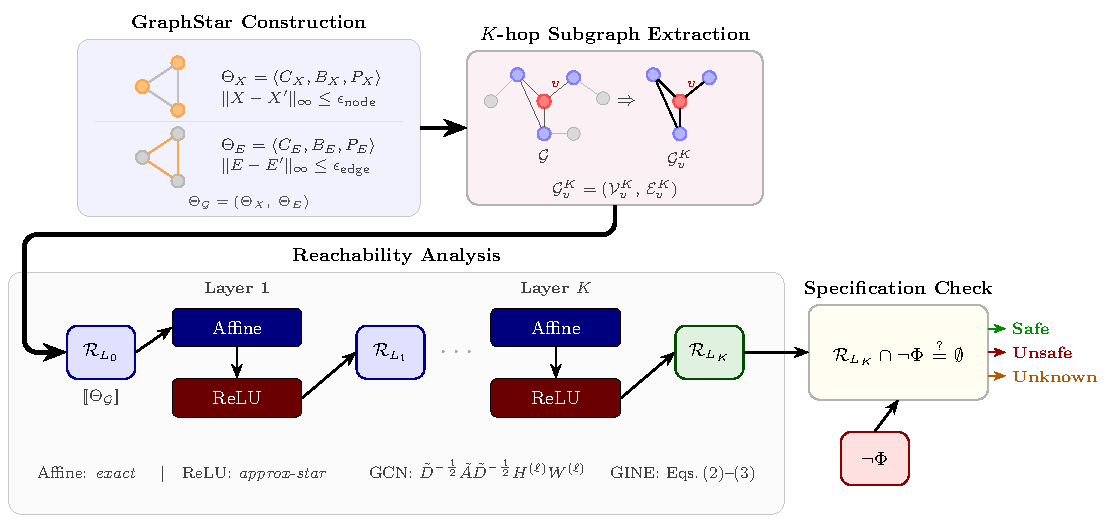
\includegraphics[width=0.91\linewidth]{figures/gnnv_pipeline_v4.pdf}
  \refline{Figure from our paper, Fig.~2.}
\end{frame}

\begin{frame}{Pipeline: GraphStar Construction to Specification Check}
  \centering
  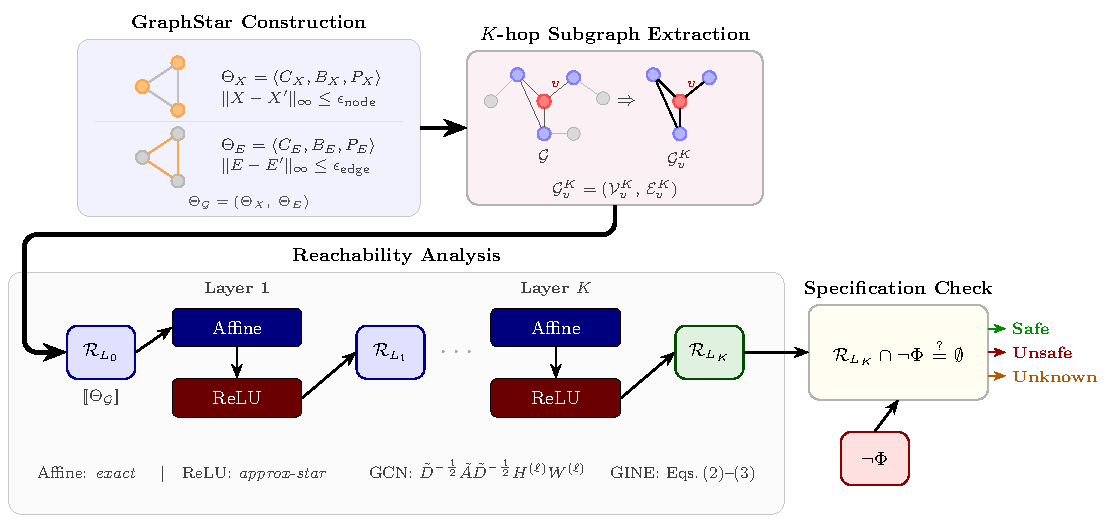
\includegraphics[width=0.64\linewidth]{figures/gnnv_pipeline_v4.pdf}
  \vskip1ex

  \begin{columns}[T,onlytextwidth]
    \begin{column}{0.235\textwidth}
      \scriptsize
      \visible<1->{\key{1. Construct.} Turn the spec
      ($\epsilon_{\text{node}}$, $\epsilon_{\text{edge}}$) into a GraphStar
      $\GS = (\Theta_X, \Theta_E)$.}
    \end{column}\hfill
    \begin{column}{0.235\textwidth}
      \scriptsize
      \visible<2->{\key{2. Localize.} Node $v$'s output depends only on its
      \textbf{$K$-hop subgraph}: verify 15 to 35 nodes of IEEE-118, not 118.}
    \end{column}\hfill
    \begin{column}{0.235\textwidth}
      \scriptsize
      \visible<3->{\key{3. Propagate.} Affine ops are \good{exact} on
      GraphStars; only ReLU is over-approximated (\textbf{approx-star}).}
    \end{column}\hfill
    \begin{column}{0.235\textwidth}
      \scriptsize
      \visible<4->{\key{4. Check.} Output set $\mathcal{R}_{L_K}$ against spec
      $\Phi$: voltage-magnitude limits (node-level regression) or
      classification robustness.}
    \end{column}
  \end{columns}
\end{frame}

\begin{frame}{Soundness and Computational Complexity}
  \begin{block}{Theorem (Soundness)}
    $f_\theta(X,A,E)\in\mathrm{Reach}(f_\theta,\GS)$\ \ for all
    $X\in\lb\Theta_X\rb$, $E\in\lb\Theta_E\rb$, for both GCN and GINE.
  \end{block}
  \vskip-0.3ex

  \begin{columns}[T,onlytextwidth]
    \begin{column}{0.50\textwidth}
      \small\textbf{The threat:} $N\!\left(Kd_h + (K{-}1)d_{\text{out}}\right)$
      ReLUs, so exact splitting is \bad{exponential}. Two levers keep it
      tractable:
      \begin{itemize}\setlength{\itemsep}{0.2ex}
        \item \key{approx-star}: LP relaxation, no case splits
        \item \key{$K$-hop locality}: queries stay local
      \end{itemize}
      \vskip0.2ex

      {\footnotesize A \key{relax-star} ablation adds \good{up to $10\times$}
      speedup at small precision loss.\par}
    \end{column}
    \begin{column}{0.47\textwidth}
      \centering
      {\footnotesize\setlength{\tabcolsep}{5pt}%
      \begin{tabular}{lcccc}
        \toprule
        s/graph & $\epsilon{=}10^{-5}$ & $10^{-4}$ & $10^{-3}$ & $10^{-2}$\\
        \midrule
        PF IEEE-24   & 0.22 & 0.24 & 0.66 & 5.1\\
        PF IEEE-39   & 0.43 & 0.63 & 2.45 & 18.5\\
        PF IEEE-118  & 1.31 & 1.47 & 2.78 & 16.9\\
        \bottomrule
      \end{tabular}}\\[0.8ex]
      {\footnotesize PF verification time per query,\\ 3-layer GINE ($d_h{=}32$).}
    \end{column}
  \end{columns}
  \takeaway{Seconds per query, even on IEEE-118 with joint uncertainty.}
\end{frame}

% ===========================================================================
\section{Experimental Evaluation}
% ===========================================================================

\begin{frame}{Experimental Setup: Benchmarks, Models, Specifications}
  \centering
  {\footnotesize\renewcommand{\arraystretch}{1.15}
  \begin{tabular}{@{}llll@{}}
    \toprule
    Task & Type & Benchmarks & Model \\
    \midrule
    PF, power flow            & node regression      & IEEE-24/-39/-118  & GINE \\
    OPF, optimal power flow   & node regression      & IEEE-24/-39/-118  & GINE \\
    CFA, cascading failures   & graph classification & IEEE-24           & GCN \\
    Protein function          & graph classification & ENZYMES, PROTEINS & GCN \\
    \bottomrule
  \end{tabular}}
  \vskip4ex

  \begin{columns}[T,onlytextwidth]
    \begin{column}{0.49\textwidth}
      \small\textbf{Specifications} $\Phi$:
      \begin{itemize}
        \item \textbf{voltage-magnitude limits} (PF/OPF): every bus/node
              stays in range, $\hat V_i \in [V_{\min}, V_{\max}]$
        \item \textbf{classification robustness}: top class invariant,
              $y_c \ge y_j\ \forall j \ne c$
      \end{itemize}
    \end{column}
    \begin{column}{0.49\textwidth}
      \small\textbf{Perturbations}:
      \begin{itemize}
        \item node $\epsilon \in \{10^{-5}, \ldots, 10^{-2}\}$,\ \
              edge $\epsilon_{\text{edge}} = 10^{-2}$
        \item 100 graphs per level; CORA compared on GCN, its supported class
      \end{itemize}
    \end{column}
  \end{columns}
\end{frame}

\begin{frame}{RQ1: Verified Robustness vs.\ Perturbation Magnitude}
  \begin{columns}[T,onlytextwidth]
    \begin{column}{0.60\textwidth}
      \centering
      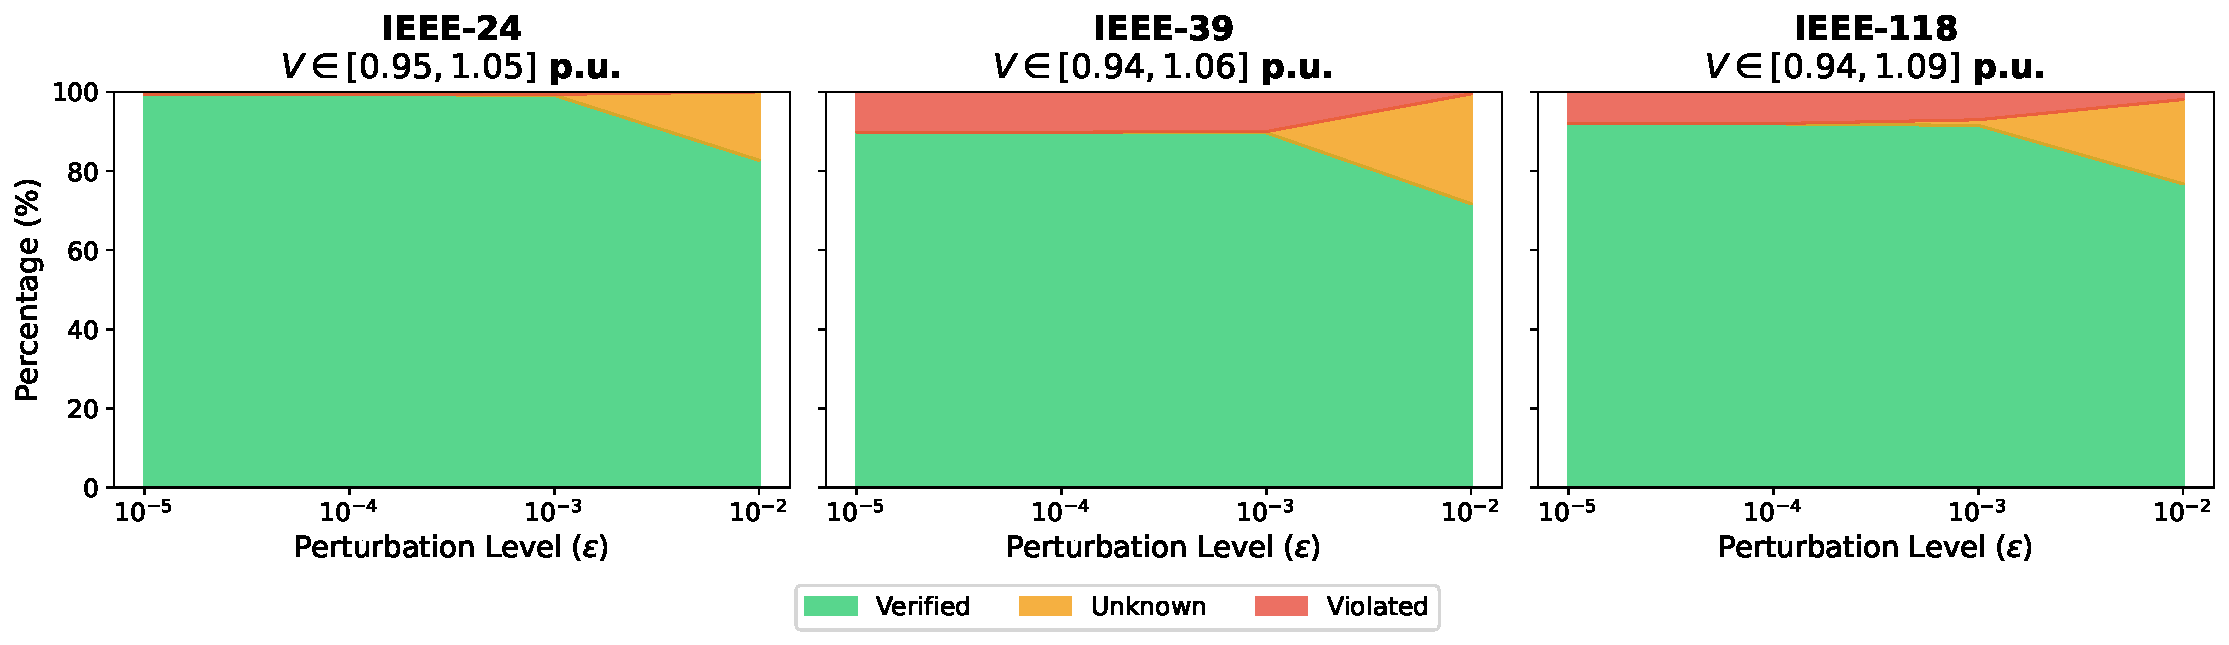
\includegraphics[width=0.98\linewidth]{figures/rq1_pf_robustness_stacked.pdf}\\[0.2ex]
      {\scriptsize PF robustness vs.\ $\epsilon$, IEEE-24/-39/-118
       (\textcolor{safegreen}{safe}/\textcolor{unsafered}{unsafe}/%
        \textcolor{amber}{unknown}); 100 graphs/level.}\\[0.8ex]
      {\scriptsize\setlength{\tabcolsep}{5pt}\renewcommand{\arraystretch}{1.1}
      \begin{tabular}{lcccc}
        \toprule
        PF, s/graph & $10^{-5}$ & $10^{-4}$ & $10^{-3}$ & $10^{-2}$\\
        \midrule
        IEEE-24  & 0.22 & 0.24 & 0.66 & 5.1\\
        IEEE-39  & 0.43 & 0.63 & 2.45 & 18.5\\
        IEEE-118 & 1.31 & 1.47 & 2.78 & 16.9\\
        \bottomrule
      \end{tabular}}\\[0.3ex]
      {\scriptsize Verification time per query (3-layer GINE, $d_h{=}32$).}
    \end{column}
    \begin{column}{0.38\textwidth}
      GINE models stay \good{highly robust} across all systems and
      perturbation levels; OPF is near-perfect.
      \medskip

      As $\epsilon$ grows, more ReLU bounds straddle zero, so some queries
      turn \textcolor{amber}{\textbf{unknown}} while verified rates stay high.
      \medskip

      $K$-hop subgraph verification keeps queries at \good{under a second} for
      small $\epsilon$ and \good{tens of seconds} at the largest~$\epsilon$.
    \end{column}
  \end{columns}
\end{frame}

\begin{frame}{RQ2: Joint Node and Edge Perturbations}
  \begin{columns}[T,onlytextwidth]
    \begin{column}{0.47\textwidth}
      {\small\renewcommand{\arraystretch}{1.25}
      \begin{tabular}{@{}lccc@{}}
        \toprule
        PF robust.\ (\%) & node only & +edge & cost\\
        \midrule
        IEEE-24  & 82.7 & 82.5 & 1.1$\times$\\
        IEEE-39  & 71.7 & 71.6 & 1.1$\times$\\
        IEEE-118 & 76.8 & 76.6 & 1.3$\times$\\
        \bottomrule
      \end{tabular}}\\[1ex]
      {\footnotesize $\epsilon_{\text{node}} = \epsilon_{\text{edge}} = 10^{-2}$.}
    \end{column}
    \begin{column}{0.49\textwidth}
      \begin{itemize}\itemsep=1.1ex
        \item robustness drop $\le 0.2\%$ across all systems, with several
              configurations showing \good{no measurable change}
        \item runtime overhead $1.1\times$ to $2.9\times$, mostly the fixed
              cost of building the edge-aware GraphStar
        \item edge generators do not grow with graph size, so overhead stays
              \good{polynomial}
      \end{itemize}
    \end{column}
  \end{columns}
  \takeaway{First edge-aware robustness guarantees: line-parameter uncertainty is now verifiable.}
\end{frame}

\begin{frame}{RQ3: Enclosure Tightness vs.\ Polynomial Zonotopes}
  \begin{columns}[c,onlytextwidth]
    \begin{column}{0.52\textwidth}
      \centering
      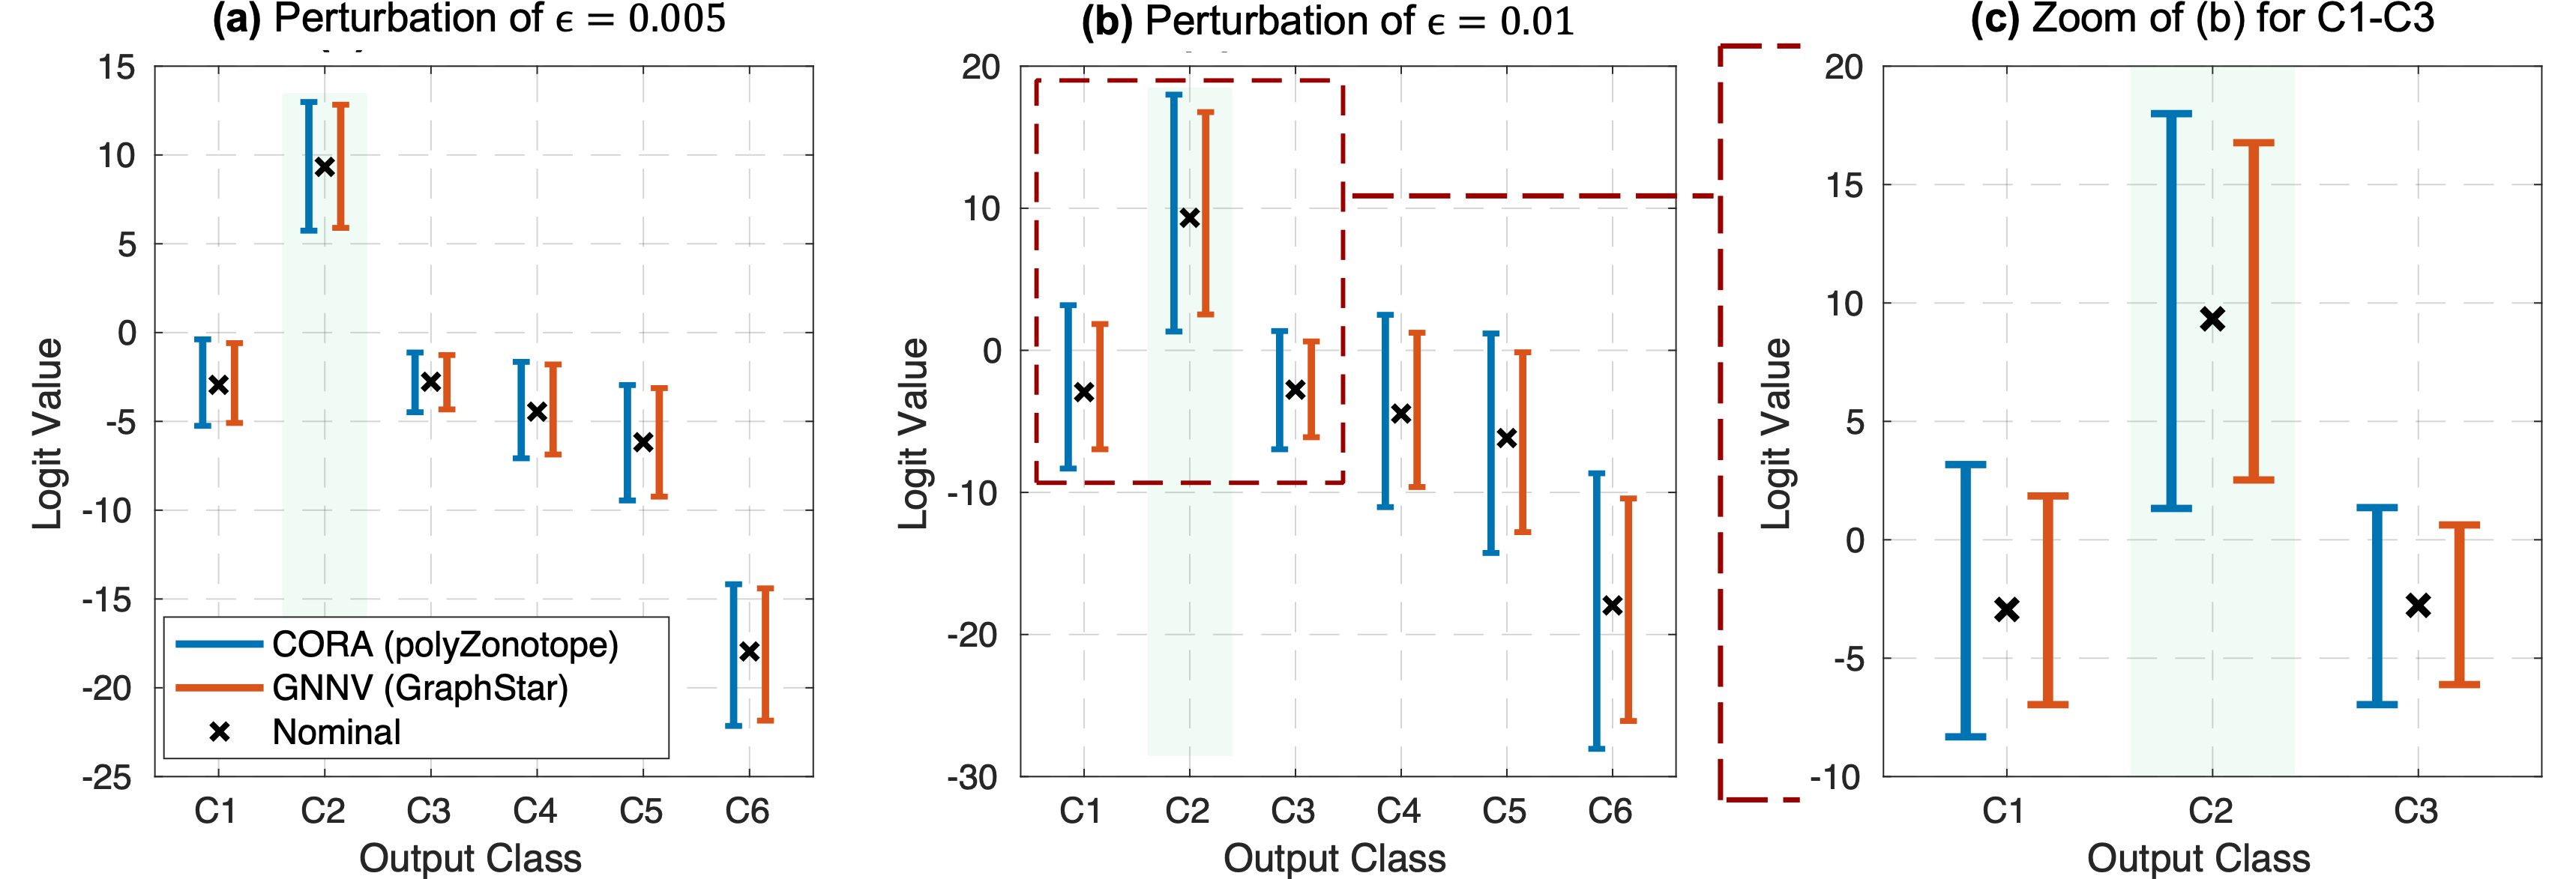
\includegraphics[width=\linewidth]{figures/rq3_enzymes_tightness.png}\\[0.4ex]
      {\footnotesize Output bounds per class, ENZYMES (GCN):
       \textcolor{steelblue}{CORA polyZonotope} vs.\
       \textcolor{VUgoldDark}{GNNV GraphStar}. At $\epsilon{=}0.01$, GNNV keeps
       class C2 \good{separated} while CORA's bounds \bad{overlap}.
       {\color{VUgrey!75}[CORA: Ladner et al., TMLR 2025.]}}
    \end{column}
    \begin{column}{0.46\textwidth}
      \centering
      {\scriptsize\setlength{\tabcolsep}{3.5pt}\renewcommand{\arraystretch}{1.15}
      \begin{tabular}{@{}lccccc@{}}
        \toprule
        & & \multicolumn{2}{c}{verified} & \multicolumn{2}{c}{s/graph}\\
        \cmidrule(lr){3-4}\cmidrule(lr){5-6}
        & $\epsilon$ & \key{GNNV} & CORA & \key{GNNV} & CORA\\
        \midrule
        ENZYMES     & .005 & \good{45/81}   & 37/81  & 8.0  & 0.16\\
        ENZYMES     & .010 & \good{9/81}    & 3/81   & 24.7 & 0.18\\
        PROTEINS    & .020 & \good{139/167} & 124/167& 16.5 & 0.14\\
        IEEE-24 CFA & .005 & \good{99/100}  & 86/100 & 0.36 & 0.03\\
        IEEE-24 CFA & .020 & \good{85/100}  & 73/100 & 1.46 & 0.03\\
        \bottomrule
      \end{tabular}}
      \smallskip

      {\footnotesize GNNV verifies \good{up to 21.6\% more graphs}: its LP
      relaxation stays tight where polynomial zonotopes accumulate error, at
      higher per-graph cost (\key{relax-star} recovers up to $10\times$).
      \par\smallskip
      \textit{Full per-$\epsilon$ tables are in the paper.}}
    \end{column}
  \end{columns}
\end{frame}

% ===========================================================================
\section{Conclusions and Tool Availability}
% ===========================================================================

\begin{frame}{Conclusions and Future Work}
  \begin{itemize}\itemsep=0.7ex
    \item \key{GraphStar sets} lift star-set reachability from vectors to
          graphs, with message passing handled \good{exactly} up to ReLU.
    \item \key{GNNV} extends NNV to GCN \textbf{and} edge-aware GINE: the
          \key{first} sound guarantees under joint node and edge
          perturbations.
    \item \good{Tighter} than polynomial zonotopes (up to \good{21.6\%} more
          graphs verified), \good{scalable} via $K$-hop locality.
  \end{itemize}
  \vskip0.6ex

  \textbf{Future directions:}
  \begin{itemize}\itemsep=0.4ex
    \item structural perturbations (edge insertion and deletion)
    \item more graph-based models and architectures
    \item a standardized \textbf{GNN verification benchmark}
  \end{itemize}
\end{frame}

\begin{frame}{Tool Availability: GNNV in NNV3 (MATLAB)}
  \vskip1ex
  \begin{columns}[c,onlytextwidth]
    \begin{column}{0.68\textwidth}
      \begin{block}{Open-source in NNV3: \texttt{github.com/verivital/nnv}}
        The \key{GNNV} module ships inside NNV3:
        \begin{itemize}\setlength{\itemsep}{0.2ex}
          \item \textbf{GraphStar} set classes (Node and Edge)
          \item \textbf{GCN} and \textbf{GINE} layer reachability with
                approx-star and relax-star
          \item robustness verification with $K$-hop subgraph extraction
          \item import of GNNs trained in PyTorch Geometric
        \end{itemize}
        \smallskip
        {\footnotesize All benchmarks, trained models, and scripts to reproduce
        RQ1 to RQ3 are included.\par}
      \end{block}
    \end{column}
    \begin{column}{0.28\textwidth}
      \centering
      \colorbox{white}{
\includegraphics[width=2.0cm]{figures/qr_nnv.png}}\\[0.2ex]
      {\scriptsize NNV on GitHub}\\[1ex]
      \colorbox{white}{
\includegraphics[width=2.0cm]{figures/qr_paper.png}}\\[0.2ex]
      {\scriptsize GNNV paper}
    \end{column}
  \end{columns}
  \takeaway{Train in PyTorch Geometric, verify in GNNV: fully open-source in NNV3.}
\end{frame}

% ---------------------------------------------------------------------------
% Thank-you page (dark)
% ---------------------------------------------------------------------------
\begin{frame}[plain]
  \begin{tikzpicture}[remember picture, overlay]
    \fill[VUblack] (current page.north west) rectangle (current page.south east);
    \node[align=center, text=white] at (current page.center) {
      {\LARGE\bfseries Thank you!}\\[1.4ex]
      {\Large\bfseries Questions?}\\[3.2ex]
      \textbf{anne.m.tumlin@vanderbilt.edu}\\[1.4ex]
      {\itshape Reachability-Based Formal Verification of Graph Neural
       Networks}\\ {\itshape with Node and Edge Features}, SAIV 2026\\[3ex]
      \begin{tabular}{cc}
        \colorbox{white}{
\includegraphics[width=1.55cm]{figures/qr_nnv.png}} &
        \colorbox{white}{
\includegraphics[width=1.55cm]{figures/qr_paper.png}}\\[0.4ex]
        {\scriptsize\color{VUgold} github.com/verivital/nnv} &
        {\scriptsize\color{VUgold} GNNV paper}
      \end{tabular}
    };
  \end{tikzpicture}
\end{frame}

\end{document}
